\subsubsection*{11.a}
On donne 2 privilegs system a admin(creation session,user) et 1 privilege objet
(select on DBAIOT.USERS) depuis DBAIOT

\lstinputlisting[style=sqlstyle]{SQL/Partie5/grant.sql}

\begin{center}
    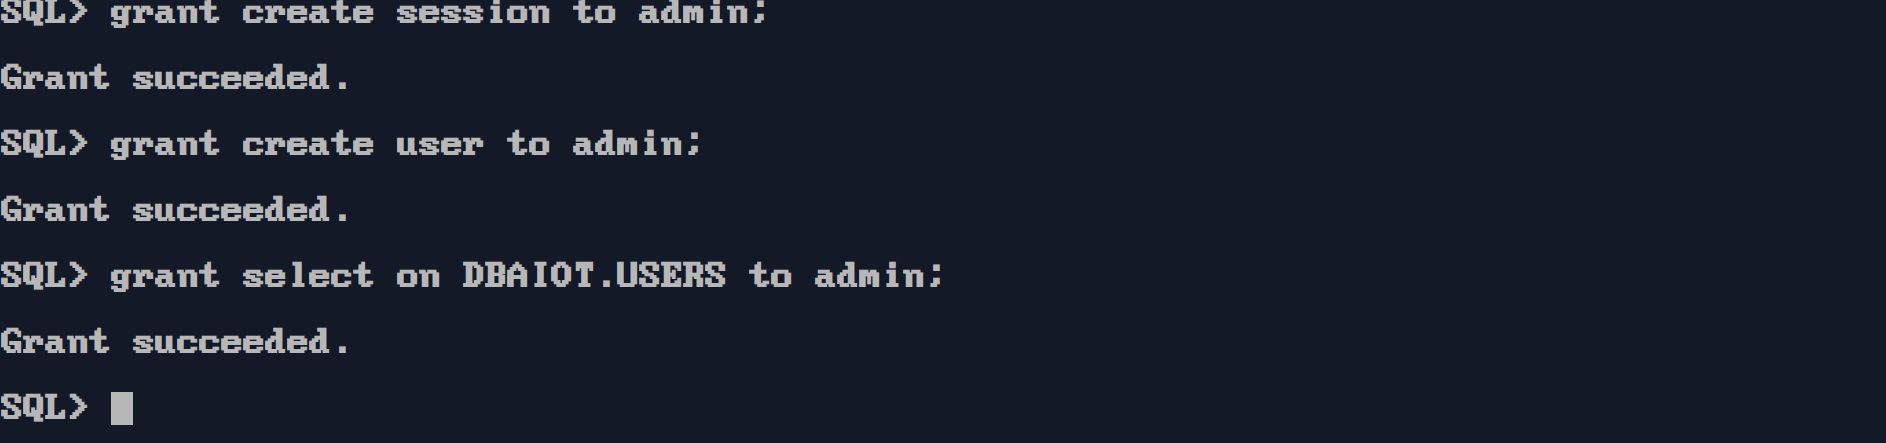
\includegraphics[width=\textwidth]{ScreenShot/Partie5/grant.png}
\end{center}

\subsubsection*{11.b}
On se connect d'abord en tant qu'admin

\lstinputlisting[style=sqlstyle]{SQL/Partie5/connectadmin.sql}

Pour afficher les privileges on va utilise la table USER\_TAB\_PRIV
pour les privileges objets et la table USER\_SYS\_PRIV pour les privileges
system 

\lstinputlisting[style=sqlstyle]{SQL/Partie5/priv.sql}

\begin{center}
    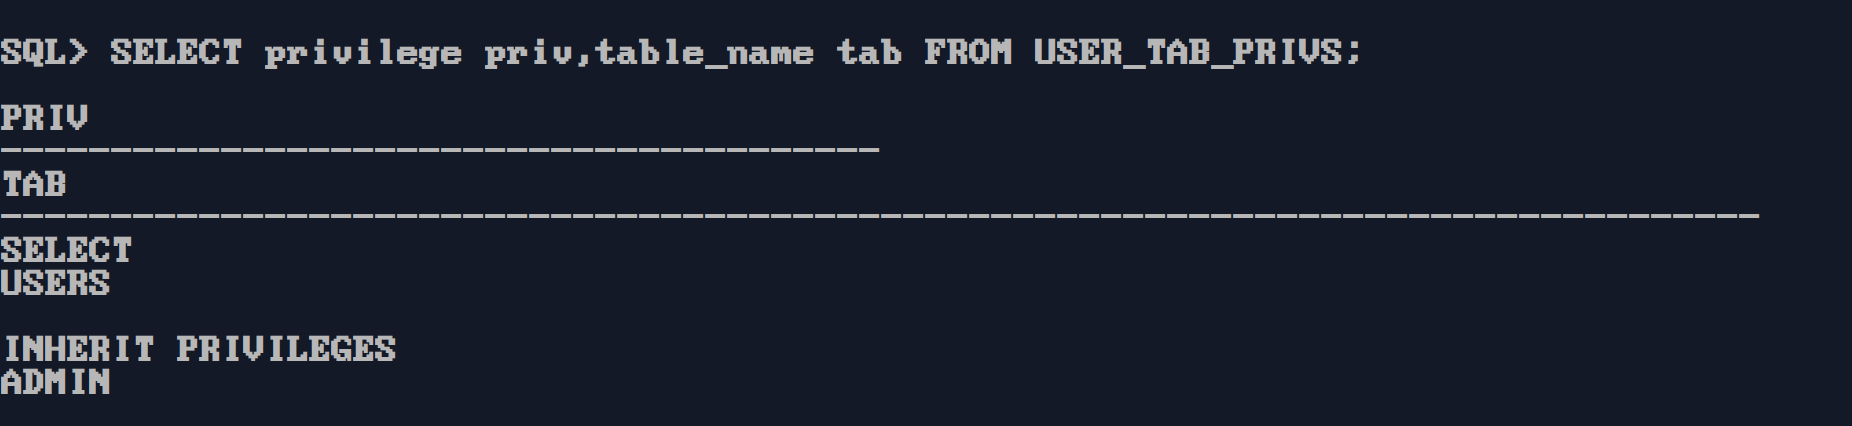
\includegraphics[width=\textwidth]{ScreenShot/Partie5/objpriv.png}
\end{center}

\begin{center}
    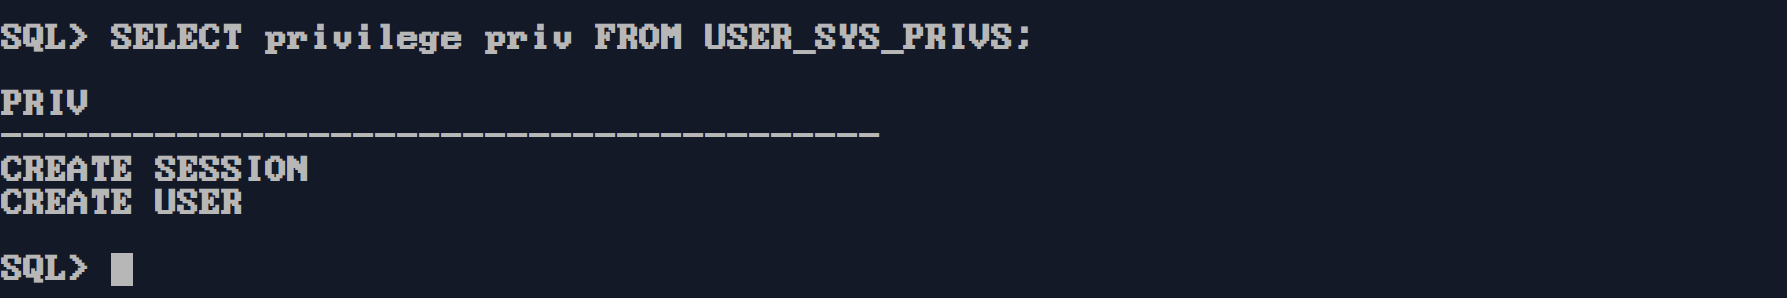
\includegraphics[width=\textwidth]{ScreenShot/Partie5/syspriv.png}
\end{center}

\begin{prettyBox}{Remarque}{myblue}
On remarque que admin a comme droits system :
\begin{itemize}
    \item creation session
    \item creation user
\end{itemize}

Et comme droits object :
\begin{itemize}
    \item select on DBAIOT.USERS
\end{itemize}
\end{prettyBox}

